% main.tex

\documentclass[conference]{IEEEtran}
\IEEEoverridecommandlockouts
\usepackage{amsmath,amssymb,amsfonts}
\usepackage{algorithmic}
\usepackage{graphicx}
\usepackage{textcomp}
\usepackage{xcolor}
\usepackage{hyperref}
\usepackage[most]{tcolorbox}
\usepackage{graphicx}
\usepackage{svg}
\usepackage{booktabs}
\usepackage{soul} % for strikethrough \st
\usepackage[numbers,sort&compress]{natbib}

\graphicspath{ {./images/} }

% Define custom colors
% \definecolor{main}{HTML}{5989cf}
% \definecolor{sub}{HTML}{cde4ff}  
% Olive color palette
\definecolor{main}{HTML}{46AF70}
\definecolor{sub}{HTML}{E2F3E9}  
\definecolor{fontColor}{HTML}{2D5B9A}
\definecolor{white}{HTML}{FFFFFF}

% Yellow highlight
\newcommand{\hly}[1]{\sethlcolor{yellow}\hl{#1}}

% Research Question Box Style
\newtcolorbox{RQBox}{
    colback = sub!50, 
    colframe = main, 
    boxrule = 0pt, 
    leftrule = 6pt
}

% Glossary box style
\newtcolorbox{GlossaryBox}{
    enhanced,
    boxrule = 0pt,
    borderline = {0.75pt}{0pt}{main},
    borderline = {0.75pt}{2pt}{sub},
    colback = white
}


% Experiment Structure Rounded Box Style
\newtcolorbox{roundedBox}{
    fontupper=\footnotesize,
    colback=sub!30,
    boxrule=1.5pt,
    colframe=main,
    rounded corners,
    arc=5pt,
    boxsep=0pt, left=0pt, right=0pt,
}

\def\BibTeX{{\rm B\kern-.05em{\sc i\kern-.025em b}\kern-.08em
    T\kern-.1667em\lower.7ex\hbox{E}\kern-.125emX}}
\begin{document}

\title{Evaluating Trade-offs of Quantized LLMs \\ for Requirements and Test Alignment}

% Evaluating Trade-offs of Using Quantized LLMs to Generate Trace Links Between Software Artifacts and Requirements In Software Projects That Utilize Traceability to Enhance Software Development --- A Comparative Experimental Empirical Investigative Analysis for the Purpose of Providing Insights

\author{
  \IEEEauthorblockN{Erik Lindstrand}
  \IEEEauthorblockA{\textit{Computer Science and Engineering} \\
  \textit{Chalmers and Gothenburg University}\\
  Gothenburg, Sweden \\
  elindstr@chalmers.se}
  \and
  \IEEEauthorblockN{Mariia Zabolotnia}
  \IEEEauthorblockA{\textit{Computer Science and Engineering} \\
  \textit{Chalmers and Gothenburg University}\\
  Gothenburg, Sweden \\
  mariiaz@chalmers.se}
  \and
  \IEEEauthorblockN{Michal Spano}
  \IEEEauthorblockA{\textit{Computer Science and Engineering} \\
  \textit{Chalmers and Gothenburg University}\\
  Gothenburg, Sweden \\
  spano@chalmers.se}
}

\maketitle

\begin{abstract}
Large Language Models (LLMs) have shown impressive capabilities (e.g., in terms of content generation, language processing) in the scientific fields of computing, software engineering, and now yield promising results in \hly{Requirements Engineering and System Testing (REST)} initiatives. However, the larger, and thus more performant, a model becomes, the more resources are required for its proper operation. As the systems we develop evolve and take in more functionality over time, associated costs grow rapidly. Fortunately, previous research discusses compression techniques, notably quantization, to decrease both training and operating costs. In this paper, we aim to investigate the impact of quantization of LLMs for generating trace links between requirements and test case artifacts. To achieve this, we conduct an experiment evaluating the rates of alignment given numerous models and their quantized counterparts. Our contributions aim to evaluate the feasibility of quantized LLMs in REST applications, focusing on efficacy, efficiency, and practical heuristics for industrial implementation.
\end{abstract}

\begin{IEEEkeywords}
Large Language Models, REST, Traceability, Quantization, Software Testing
\end{IEEEkeywords}

\section{Introduction}\label{sec:intro}

The modeling of human language---a long-established field within science---has particularly seen its rise with the introduction of web- and transformer-based chatbots (e.g. ChatGPT, DeepSeek) \cite{jones1994Natural,vaswani2017Attention,naveed2024Comprehensive}. Since then, science, education, and medicine have all made use of LLMs that employ the transformer architecture. Moreover, LLMs have been exceptionally helpful in Software Engineering tasks \cite{naveed2024Comprehensive}; notably in requirements engineering \cite{arora2024Advancing} or software testing \cite{dakhel2024Effective, wang2024Software}. In particular, Ivarsson and Setterström have demonstrated that LLM-assisted trace link generation is feasible and yields satisfactory results \cite{ivarsson2023automated}. This claim is further supported by a study of Quinstedt and Lindgren who developed the \verb|REST-at| tool that this study builds upon \cite{quinstedt2024Optimizing}. 

Given the growing size and complexity of software systems, the coordination of work and artifacts is oftentimes challenging. As a result, researchers and practitioners identify \textbf{trace links} between software and development artifacts to manage this complexity \cite{jaber2013Effect}.

Research and development in LLMs are advancing rapidly, along with their performance capabilities. Typically, a more performant model requires more computational resources due to an increased number of model parameters, leading to financial and environmental concerns \cite{naveed2024Comprehensive}. Fortunately, there exist well-established strategies to mitigate the hardware requirements necessary to load and run LLMs, and one that particularly interests us is \textbf{quantization} (c.f. \cite{shen2024exploring, frantar2023GPTQ, lin2024AWQ, chen2024EfficientQAT}). 

Given the exponential growth in terms of cost, there is an incentive to improve the efficiency of LLM tools, e.g. through quantization methods, to better utilize automated trace generation tools at scale. Therefore, the purpose of this study is to evaluate the \textbf{efficacy} of quantized models when used to generate REST trace links. Furthermore, the trade-off analysis will consider the \textbf{efficiency} of the models, which is a consequence of model size and hence affected by the quantization that is applied.

\begin{RQBox}
    \textbf{RQ1}: How do quantized LLMs perform compared to non-quantized LLMs
    in terms of \textbf{efficacy} when used to create REST trace links?\\[0.5em]
    We will evaluate model efficacy using the following metrics: \textit{accuracy, precision, recall, F1-score}
\end{RQBox}


\begin{RQBox}
    \textbf{RQ2}: How do quantized LLMs perform compared to non-quantized LLMs in
    terms of \textbf{efficiency} when used to create REST trace links? \\[0.5em]
    We will evaluate model efficiency using the following metrics: \textit{time-to-analyze, GPU memory usage (vRAM)}.
\end{RQBox}

\begin{RQBox}
    \textbf{RQ3}: What are the trade-offs of using quantized LLMs for REST alignment
    with respect to efficacy versus efficiency? \\[0.5em]
    We are particularly interested in investigating whether it is possible to balance acceptable recall and F1-score with lowered memory usage.
\end{RQBox}


% Encapsulated footnote for reusing in several places 
\newcommand{\modelsFootnote}{In this paper, a ``baseline'' model is one of the following: Mistral 7B Instruct-v0.2 (i.e., Mistral), Mixtral 8x7B Instruct-v0.1 (i.e., Mixtral), and LLAMA 3 70B-Instruct (i.e., LLAMA 3).} 

Our findings arise from an experiment where we compare the generated trace links from each model against the \textit{ground truth} provided by our industry partner TestScouts\footnote{\url{https://testscouts.se/}}.\footnote{The ground truth essentially stands for the desired mapping of requirements and tests, established by the respective company.} We generate trace links with each model using the \verb|REST-at| tool which we run on \verb|Alvis|, a cloud platform for scientific computing\footnote{\url{https://www.c3se.chalmers.se/about/Alvis}}. We access both the baseline\footnote{\label{baselineModels}\modelsFootnote} and quantized models from public repositories hosted on \textit{HuggingFace}\footnote{\url{https://huggingface.co/}}.

Our scientific contributions include: evaluating the feasibility of quantized LLMs for REST in terms of efficacy and efficiency metrics; examining the trade-offs, such as the practicality of use and how efficacy is affected when optimizing for lower operational costs. Furthermore, our technical contributions include revising REST-at to support quantized models as well as updating the tool to comply with other technological changes that are affecting its use and have been introduced since it was developed. Additionally, we aim to provide guidelines for implementing quantization in industrial REST applications.

\section{Background \& Related Work}\label{background}

\subsection{Requirements Engineering and System Testing Alignment}

REST \st{(Requirements Engineering and System Testing)} alignment has been the subject of prior research studies, as has been shown in systematic literature mappings \cite{barmi2011Alignment, karhaapa2017What}. Achieving REST alignment involves activities that coordinate Requirements Engineering and System Testing efforts in order to optimize product development \cite{unterkalmsteiner2014Taxonomy}. Traceability is one of the tools that can be used to achieve alignment through the structuring of artifacts, such as requirement specifications and test cases, by creating connections (or traces) that help to evaluate and improve requirements coverage \cite{bjarnason2014Challenges}. Jaber et al. define a trace link as any link between different artifacts, such as a particular \textit{code element} (e.g., software test) in relation to a \textit{design element} (e.g., requirement specification) \cite{jaber2013Effect}. 

Real-world challenges in aligning RE and ST practices have been examined in previous case studies \cite{bjarnason2014Challenges,gomes2017Challenges}. According to both Bjarnason et al. and Gomes et al., introducing tracing between requirements and test cases is costly, meanwhile, a lack of traceability also comes with significant additional cost. There is also significant challenge in updating and maintaining traces between RE and ST artifacts, e.g., when requirements change. Moreover, the case study by Bjarnason et al. identifies a need, among the companies involved in the study, for tools that can manage REST traceability artifacts \cite{bjarnason2014Challenges}.

\subsection{Automated REST Alignment Using LLMs} 

There have been studies on the development of more advanced tools to aid in the trace creation process, with Ivarsson and Setterström showing promise in automating the process using LLMs by leveraging OpenAI’s GPT-3.5-turbo model\cite{ivarsson2023automated}. Their tool achieved an average of 86.394\% across accuracy and recall, although with limitations in terms of precision with an average of 45.582\%. Notably, the computational complexity is nonlinear in relation to the input size (requirements + test cases), resulting in an exponentially growing cost both financially and in \textit{time-to-analyze}, i.e., returning the results (trace links), which negatively impacts scalability \cite{ivarsson2023automated}. Furthermore, the study by Ivarsson and Setterström included identifying the main requirements for an automated REST tracing tool by performing literature reviews as well as conducting interviews with practitioners working at TestScouts, a company specializing in software testing \cite{ivarsson2023automated}.

Building on the work of Ivarsson and Setterström, Quinstedt and Lindgren conducted a study in which they evaluated and compared the efficiency of several different LLMs in creating REST trace links \cite{quinstedt2024Optimizing}. The requirements identified in Ivarsson and Setterström's study \cite{ivarsson2023automated} were further refined in collaboration with the same industry partner, TestScouts. These requirements were then used to develop a tool called \textit{REST-at} (REST alignment tool) which is capable of creating REST trace links by interfacing with proprietary models, such as OpenAI's GPT-4, through the use of APIs, in addition to using non-proprietary locally stored LLMs. Importantly, their study showed that smaller LLMs (in terms of number of parameters) were capable of achieving comparable results with much larger LLMs, with LLAMA 3 (70B parameters) achieving a 100\% recall score on the GBGE dataset, compared to GPT-3.5 (175B parameters) which had a recall score of 90.87\%.

However, Quinstedt and Lindgren's study also identified a key challenge in regards to hardware requirements and cost, due to the fact that running the LLMs require substantial computational resources. For instance, running the previously mentioned LLAMA 3 model with its 70B parameters requires 140 GB vRAM \cite{quinstedt2024Optimizing}. In order to mitigate this challenge, the study had to be adapted to instead run the models on the Alvis research cloud  infrastructure, offering significantly more computational power.

Given the challenges faced due to hardware constraints when utilizing LLMs, there is a need to explore techniques that would reduce the GPU memory usage. Moreover, it is still unclear whether using quantized models is useful for the purposes of REST alignment. Hence, we identify a gap in the current research regarding the application of quantized LLMs for the purpose of REST alignment. Thus, we will explore LLM quantization methods as a viable technique to allow for models to run in a non-cloud environment while retaining reasonable performance in terms of automating REST traceability.

\subsection{Quantization of LLMs}

Quantization is one of the LLM compression techniques, along with pruning, knowledge distillation, and low-rank approximation\cite{bai2024beyond}. It stands out for its ability to directly reduce memory usage while maintaining reasonable accuracy and performance of LLMs. Some studies even report a notable acceleration of the inference latency for quantized models\cite{shen2024exploring}.

Drawing a parallel to common image compression principles (cf. Figure \ref{fig:quantvisual}), quantization is performed, in essence, by converting the weights and activations from a high-precision data representation to a reduced-precision format \cite{zhao2025benchmarking, bai2024beyond}. This is illustrated by transforming the FP32(32 bits) number to, for example, INT8(8 bits), which is particularly impactful at the scale of billion parameters, enabling smaller-size model execution on resource-constrained devices.

\begin{figure}[ht]
    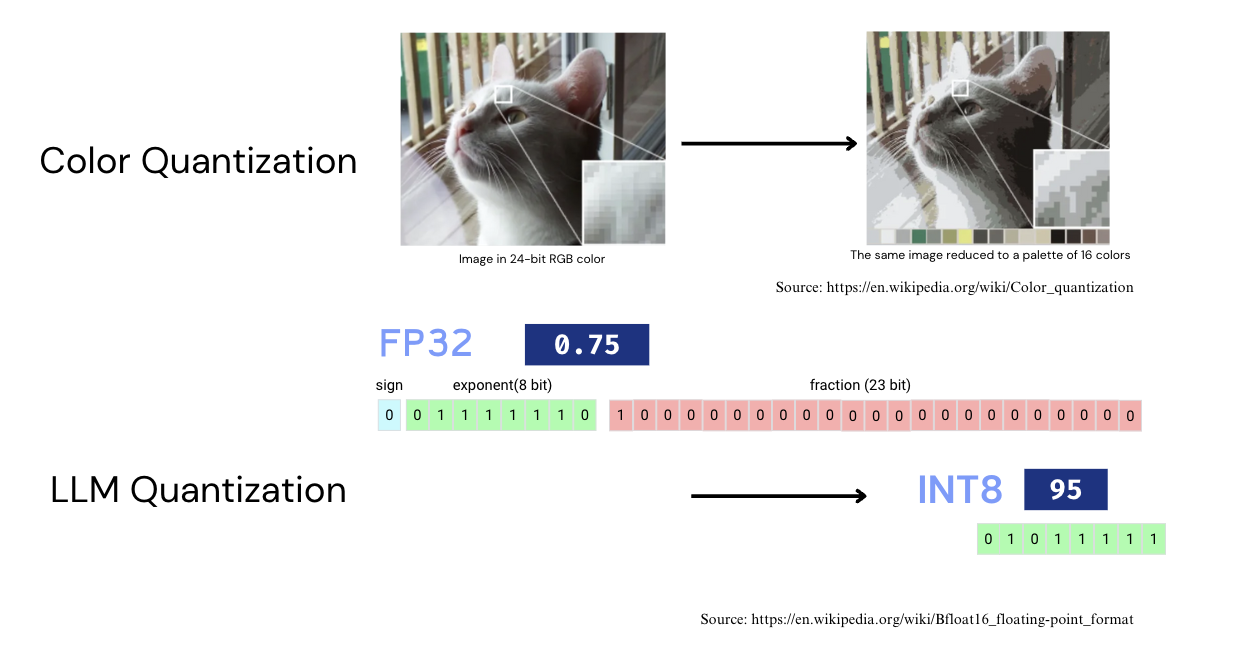
\includegraphics[width=\columnwidth]{img}
    \caption{Analogy between color quantization and LLM quantization}
    \label{fig:quantvisual}
\end{figure}

Quantization can be applied 1) during the training phase (\textit{QAT}) which is observed to be highly efficient; however, due to significant resource demands, oftentimes appears impractical \cite{chen2024EfficientQAT}, and 2) post-training (\textit{PTQ}), which is more resource efficient, but can lead to certain levels of performance degradation \cite{shen2024exploring}. An important quantitative marker of precision loss, quantization error, is often used to assess the degree of approximation loss \cite{lin2024AWQ}.

Having established the theoretical foundation of quantization, we now provide an overview of key methods. \textit{GPTQ} (Generative Pre-trained Transformers Quantization) focuses solely on weights and aims to minimize quantization error through optimal weight rounding. It is almost twice as effective as its one-shot predecessors and is capable of quantizing a 175 billion parameter model in a few hours with minimal accuracy loss\cite{frantar2023GPTQ}. \textit{AWQ} (Activation-aware Weight Quantization) assumes that weights carry varying levels of importance; therefore skipping crucial activation outliers while aggressively quantizing the rest helps mitigate accuracy loss. It also shows approximately 3x faster inference speed on a desktop, even allowing deployment and execution of a 13-billion model on a laptop with 8GB of RAM, which is of high interest for our study \cite{lin2024AWQ}. \textit{GGUF} (GPT-Generated Unified Format), in turn a successor of the deprecated \textit{GGML} (GPT-Generated Model Language), includes  quantization-aware kernels optimizations and  provides backward-compatible file format among other improvements. By offering such features as single-file deployment and improved loading and saving speed, it introduces a smoother workflow for forking with LLMs \cite{rajput2024benchmarking}. \textit{SmoothQuant} \cite{xiao2023SmoothQuant} enables quantization for both activations and weights by managing outlier values and QLoRA (4-bit quantized version of LoRA fine-tuning technique) \cite{dettmers2023qlora} reduces GPU requirements while still preserving performance.

% The described approaches demonstrate not only superior advancements and efficiency, but are also feasible for us to experiment with. Therefore, in this study, we plan to quantize each of the baseline models\footnotemark[\getrefnumber{baselineModels}] using the GPTQ, GGUF and AWQ techniques to reduce model size \footnote{By ``size'' we refer to bit width which in turn affects the needed memory for execution} to mitigate hardware requirements. Later we employ them to generate REST trace links, analyze their performance, and answer our RQs.

The described approaches demonstrate not only superior advancements and efficiency, but are also feasible for us to experiment with. Therefore, in this study, we plan to access models from HuggingFace that have been quantized using the following techniques: GPTQ, \st{GGUF} and AWQ. These approaches reduce model size\footnote{By ``size'' we refer to \textit{bit width} which in turn affects the memory needed for execution} to mitigate hardware requirements. Later we employ them to generate REST trace links, analyze their performance, and answer our RQs. 

\section{Research Methodology}\label{sec:method}

% TODO: Mention something here about insecure quantization (see Exploiting quantization). -> WHY we consider quantization on our own.

This section outlines the research type and its design (cf. Figure \ref{fig:method-overview}), and defines the scope pertaining to identified RQs. We structure our methodology section following the experimental process recommended by Wohlin et al. \cite{wohlin2012experimentation}. Furthermore, we explain and motivate the choice of methods and statistical tests for data analysis. Lastly, we acknowledge identified validity threats accompanied by mitigation strategies.

We perform an \textit{experiment}, a research method commonly used to explore empirical correlations between several factors, in our case, LLM models and quantization techniques. Given the nature of  experiments, we gain control over subjects, objects, and instrumentation in order to operate on experimental units and draw conclusions on dependent variable output. Experiments are conducted to test the hypotheses and comparatively assess the impact of specific variables in a controlled setting, which is the most suitable setup for answering our RQs.

\begin{figure}[h]
    \centering
    \includesvg[width=\columnwidth]{method-overview-refined.svg}
    \caption{Overview of the research methodology process}
    \label{fig:method-overview}
\end{figure}

\subsection{Scope and Planning}
We define the scope of our experiment using the said framework of Wohlin et al. \cite{wohlin2012experimentation}. That is, we analyze quantized LLMs for the purpose of evaluation with respect to their efficacy, efficiency, and practicality from the point of view of developers and/or managers in the context of industry REST alignment initiatives.

We will conduct a full factorial controlled experiment. There are two factors in our study: baseline models\footnotemark[\getrefnumber{baselineModels}] and quantization approaches. There are three levels for the models: LLama, Mistral, and Mixtral; and \hly{three levels for the quantization}: \textit{None}, GPTQ, \st{GGUF} and AWQ. We generate \st{$3 \times 4 = 12$} $3 \times 3 = 9$ treatments. Our choice of models is based on the previous work of Quinstedt and Lindgren \cite{quinstedt2024Optimizing} as they opened up the questions explored in our study; thus aligning the model selection with their study allows for a more detailed and direct trade-off comparison.

The dependent variables reflect the definition of performance in this study; they are: accuracy, precision, recall, and F1-score (RQ1, efficacy), as well as time-to-analyze and GPU memory-usage (RQ2, efficiency).

Our control variables include requirements specification and test case files, as well as the ground truth which specifies the correct trace links between tests and requirements. This data comes from two datasets: the first has been provided to us by our industry partner and originates from G\"oteborg Energi, the second was sourced from Bluetooth Headset Profile 1.2\footnote{\url{https://www.bluetooth.com/specifications/specs/headset-profile-1-2/}}. Additionally, our control variables include a prompt template which will be used with the REST-at tool evaluated in a previous study \cite{quinstedt2024Optimizing}. They found that various prompt templates lead to fluctuations in the results; therefore we have selected the most performant one. Furthermore, model hyper-parameters will be kept constant and configured to be as similar as possible between different models, such as model \textit{temperature} that controls the randomness of an LLM's output. We also standardize the Python environment (version) as it has a direct impact on code execution speeds and therefore also on our results.

An overview of the experimental design can be found in Figure \ref{fig:exp-design}. See subsection \ref{sec:instrumentation} for further specification of the experiment objects.

%%%%%%%%%%%%%%%%%% HYPOTHESIS TABLE %%%%%%%%%%%%%%%%%%

\newcommand{\equalM}{$M_{1} = \dots = M_{12}$}
\newcommand{\notEqualM}{$M_{1} \neq \dots \neq M_{12}$}

\begin{table}[h]
    \centering
    \caption{Experiment Hypotheses}
    \renewcommand{\arraystretch}{1.65} % original value 1.5
    \begin{tabular}{@{} c p{3.5cm} p{3.5cm} @{}}
    \toprule
    &\multicolumn{1}{c}{\textbf{(i) Efficacy RQ1}}
    &\multicolumn{1}{c}{\textbf{(ii) Efficiency RQ2}} \\
    \midrule
    $H_{0}$ % <-- NULL HYPOTHESIS %
    & There is no difference in \textbf{efficacy} between the treatments
    under test; \equalM.
    & There is no difference in \textbf{efficiency} between the treatments
    under test; \equalM.\\
    $H_{a}$ % <-- ALT HYPOTHESIS %
    & There is a difference in \textbf{efficacy} between the treatments
    under test; \notEqualM.
    & There is a difference in \textbf{efficiency} between the treatments
    under test; \notEqualM.\\
    \bottomrule
    &\multicolumn{2}{c}{Note: the individual treatments are labeled as $M_{1\dots12}$.} \\
    \end{tabular}
    \label{tab:hypothesis}
\end{table}

First, we will collect data and derive metrics from repeated test iterations. The process is repeated on \hly{all datasets with 10 repetitions per treatment; we altogether obtain $4 \times 9 \times 10 = 360$ output artifacts} containing trace links. When analyzing the data, we will initially examine the treatments from two perspectives: (i) efficacy, and (ii) efficiency---evaluating the null hypotheses for these groups of metrics separately (cf. Table \ref{tab:hypothesis}). After testing for our null and alternative hypotheses, we apply a post-hoc pairwise comparative analysis of the treatment pairs. Finally, a descriptive analysis will investigate trade-offs of using quantized LLMs for REST alignment; we will combine the results from both efficacy and efficiency metrics, as well as some additional factors (e.g., implementation challenges, learning curve) that are described in detail in subsection \ref{sec:analysis}. 

%%%%%%%%%%%%%%%%%% EXPERIMENTAL DESIGN FIGURE %%%%%%%%%%%%%%%%%%

\begin{figure}[h]
\begin{center}
    \begin{tcbraster}[raster columns=2, raster column skip=5pt, raster equal height=rows, raster row skip=5pt]
        \begin{roundedBox}
            \centering
            \textbf{Independent Variables \& Levels}
            \begin{itemize}
                \item Model:
                \begin{itemize}
                    \item LLama
                    \item Mistral
                    \item Mixtral
                \end{itemize}
                \item Quantization technique:
                \begin{itemize}
                    \item None
                    \item GPTQ Quantization
                    \item \st{GGUF Quantization}
                    \item AWQ Quantization
                \end{itemize}
            \end{itemize}
        \end{roundedBox}
        \begin{roundedBox}
            \centering
            \textbf{Objects}
            \begin{itemize}
                \item Hardware (Alvis)
                \item Alvis job-scripts
                \item REST-at tool
                % \item Hardware: local
            \end{itemize}
        \end{roundedBox}
        \begin{roundedBox}
            \centering
            \textbf{Dependent Variables}
            \begin{itemize}
                \item Accuracy
                \item Precision
                \item Recall
                \item $F1$-score
                \item Time-to-analyze
                \item GPU memory-usage (vRAM)
            \end{itemize}
        \end{roundedBox}
        \begin{roundedBox}
            \centering 
            \textbf{Control Variables}
            \begin{itemize}
                \item Requirements file
                \item Test case file
                \item Ground truth file
                \item Prompt template
                \item Model hyper-parameters
                \item Python environment (version)
            \end{itemize}
        \end{roundedBox}
        \end{tcbraster}
        \begin{roundedBox}
            \centering
            \textbf{Output (artifacts)}
            \begin{itemize}
            \centering
                \item Structured trace links
            \end{itemize}
        \end{roundedBox}
    \caption{Overview of the experimental design}
    \label{fig:exp-design}
\end{center}
\end{figure}

\subsubsection{Instrumentation}\label{sec:instrumentation}
For our instrumentation, we extend REST-at by adding support for (i) quantized models, and (ii) logging efficiency data from the models' execution. We run our experiment on Alvis, a cloud platform for scientific computing. The system is built around multiple NVIDIA GPUs, and allows executing jobs on demand. Therefore, we execute the experiments on a dedicated set of available NVIDIA A100 Tensor Core GPUs\footnote{\url{https://www.nvidia.com/en-us/data-center/a100/}}, which inherently makes all performance and efficiency metrics rely on this hardware configuration.

For our experiment, we require a set of requirements linked with a corresponding set of tests. The datasets with trace links serve as \textit{ground truth} since these are established by the authors from the companies.

% In addition, we plan to search for more datasets in \textit{Zenodo}\footnote{\url{https://zenodo.org}} from existing research and open-source projects. 

\subsubsection{Sampling and Data Collection}
The requirement and software test pairs are sampled from each dataset to create subsets ranging from \hly{30 through 40} items using PRNG\footnote{Pseudo-random Number Generator, cf. \url{https://epubs.siam.org/doi/abs/10.1137/0215025}}. This sampling also has the benefit of reducing overall computational costs. No human subjects are involved in this phase beyond the authors of this paper, who oversee the experiments in the event of technical difficulties.
% TODO: expand more on subsets and how we plan to use them (this is most likely to be discussed after the progress meeting because it adds more complexity).

Note that, given the stochastic nature of LLMs, it is important that we perform repeated tests on the same input for each of the treatments in order to include standard deviation measurements across the different metrics; for this reason, we will perform 10 repetitions for each treatment. This will allow us to reason about the consistency of each treatment as well as increase the validity of our measurements and subsequently the results of our analysis.


\subsection{Analysis and Interpretation}\label{sec:analysis}

The data analysis includes performance indicators from a confusion matrix: accuracy, precision, recall, F1-score. Those measures convey the efficacy of the treatment under test. We derive the mean, median, and standard deviation from the (repeated) tests for each treatment to give reliable measurements for all the different metrics. 

Our full factorial design has two factors. The data is paired as we will be comparing the same data points (rows) between different treatments. First, we will analyze the distribution of the collected data. \hly{Specifically, we will use the Shapiro-Wilks test to check for distribution normality and Levene's test to check for homoscedasticity}---equal or similar variance between groups. If these tests show that necessary assumptions are met, we will use a parametric two-way ANOVA statistical test. If the assumptions do not hold, we will instead use a non-parametric Friedman test which is an alternative to repeated ANOVA-measures \cite{mccrum2008statisticalTests}.

%First, we analyze the collected data using the Kruskal-Wallis statistical test: collected data is non-parametric---there are no assumptions about its distribution---and paired---we are comparing the same data points (rows) between different treatments \cite{wohlin2012experimentation}. % RIP IN PIECE MY SWEET PRINCE ;_; KRUSKWALL 1952-2025

Should the null hypothesis be rejected, indicating that there is a significant difference between at least one of the treatment pairs, we conduct a pairwise post-hoc analysis to identify the differing pairs as well as in which direction they differ. By evaluating the treatment pairs, we can examine whether certain quantization techniques result in better model performance within the given context. 
%The z-score based Dunn's test will be used for the post-hoc analysis, as the sample size is $>$30 \cite{dunn1964dunnTest}. 
% Can also mention that it is a rank-based follow-up test to Kruskal-Wallis - if we can find a source ... -_-
% ...or the Conover-Iman test \cite{conover1979conoverImanTest} will be used depending on the sample size. 
% NOTE: keeping this here since we might use this test instead (it has better statistical power)? Also, is it okay that we cite the original sources here and not literature that recommends the test's usage?
We use the Holm–Bonferroni method to mitigate \textit{alpha inflation} which would otherwise increase the risk of type I errors---while also reducing the risk of type II errors compared to the regular Bonferroni method \cite{abdi2010HolmBonferroni}.
Note that we will decide the appropriate post-hoc test method at a later stage and update this section accordingly.

We conduct a descriptive statistical analysis of the results to analyze and discuss the trade-offs of applying quantization to LLMs within the given context. We are particularly interested in examining whether there exists any treatment(s) that retains acceptable / usable recall and F1-score results despite significantly reducing GPU memory-usage. Thus, we combine the efficacy and efficiency metrics alongside the following additional factors: implementation challenges, learning curve, model vRAM usage compared with commercial GPU alternatives, cost comparison of manual and automatic solutions. 

We choose to represent the data in tables comparing the results from the different treatments. For this purpose, \textit{mean $\pm$ standard deviation} is displayed for each of the relevant metrics. We also select box-plots in order to visualize the distribution as well as any outliers in each treatment's performance. Lastly, we use bar charts to give a clear comparison of the performance as a result of the different quantization techniques.

\subsection{Threats to Validity}
% - Describe internal validity threats and mitigations.
% - Describe construct validity threats and mitigations.
% - Describe external validity threats and mitigations.
% - If applicable for your research method, describe further validity threats and mitigations under further categories.

Based on the guidelines proposed by Wohlin et al. \cite{wohlin2012experimentation} we identify the following threats to validity that might have influenced our research findings: 
\subsection*{\textbf{1) Internal validity}}
    \textit{Response variability}: due to stochastic behavior of LLMs, the same prompt can result in different outputs when executed several times; we mitigate this risk by invoking prompts multiple times and defining consistent hyperparameters.

    \textit{Selection of models}: in this study, we select open-weight, state-of-the-art LLMs representative of a common choice among practitioners. This selection also leverages on the previous research by Quinstedt and Lindgren \cite{quinstedt2024Optimizing}, which we are building on. Aligning the selection of LLMs with their results allows for a more extensive and direct trade-off comparison. More models can be explored in future work, and we provide instrumentation in the Methodology section to facilitate the smooth integration.

    \textit{Quantized LLM quality}: we have utilized quantized models distributed via the \textit{HuggingFace} platform. While there is a risk in depending on quantized models from a third-party service, HuggingFace is one of the main sources for developers or organizations to download and/or deploy open weight models. As such, these models are likely to be used by practitioners, meaning that the results of our study are representative of the real-world use of quantized LLMs, given that this assumption holds.

\subsection*{\textbf{2) External validity}}
    
    \textit{Domain-Specific Applicability}: our study evaluates quantized LLMs within the specific use case of REST alignment. Exploring the trade-off of quantization in using LLMs for other Software Engineering tasks is beyond the scope of our thesis; however, it could be explored in future work.

\subsection*{\textbf{3) Construct validity}}

\textit{Ground Truth Validity}: the REST alignment mappings that are used in this study as ground truth have been obtained from our Industry Partner (specializing in software testing) \hly{and public online resources, and hence are representative} of software artifacts in industry. However, any potential human bias, error, or other factors influencing the creation of these trace links could have an impact on the results of this study/experiment.

\st{\textit{The need for more datasets}: in this study we are using two datasets to evaluate the tradeoffs of using quantization. However, incorporating more datasets could provide a broader perspective and improved generalization of the results, opening up new opportunities for future research to validate obtained results across different contexts.}

\section{Preliminary Results \& Findings}

This newly added section discusses the team's progress since the submission of the \textbf{thesis proposal} (dated March 14, 2025). Furthermore, changes to the previous section are highlighted in \hly{yellow} (additions) or with a \st{strikeout} (deletions).

\subsection{Stabilized Environments}

Much of AI/ML programming depends on third-party libraries, which evolve rapidly and often rely on pinned versions of other dependencies. To maintain stability, we have defined consistent environments for the quantization methods under consideration, as well as for REST-at. This ensures the pipeline can run on Alvis without any dependency conflicts. 

However, despite our best efforts, GGUF has proven to be particularly challenging to realize in our pipeline (notably due to the fact that it operates fundamentally differently and isn’t truly a quantization ``method'' in the traditional sense) and we're considering removing it from our scope.


\subsection{Alvis pipeline for model prompting and data processing}\label{sec:progress-alvis-pipeline}

We have set up a pipeline to automate iterative REST alignment experiments on Alvis. It streamlines the process by running the experiments and saving the results iteratively  inside Alvis. This is a crucial step because it provides the necessary data used for further statistical analysis.
%To setup the experiment, the user must provide a dataset, model definitions, and quantization parameters. The processed results are generated and saved in the following directory structure: \verb|M_Q_D/date/timestamp/ITER_NUM/res.json|,  where \verb|M| represents the model name, \verb|Q| the quantization configuration, and \verb|D| the dataset.

\subsection{GPU Profiling}

We are in the process of incorporating an extension of the Alvis pipeline which is capable of monitoring the GPU instance during a job execution using the \verb|nvidia-smi|\footnote{\url{https://developer.nvidia.com/system-management-interface}} utility. This interface enables us to extract parameters such as GPU utilization and maximum allocated GPU memory (vRAM) with very little overhead and in real-time.

%This extension is accompanied with an additional script file that (i) reads the data entries to memory, (ii) computes job-specific metrics and populates the previously acquired metric files, and (iii) (optionally) visualizes the evolution over the job lifespan (and this has proven to be very useful when tracing bugs). See below for an example invocation with in the ``visualizer'' mode.

This extension allows us to optionally visualize the GPU and vRAM utilization across a job (iteration) execution. The generated graph shows utilization as a percent of the available resources (Y-axis) over the samples taken over time (X-axis). See below for an example from a test run---note that the top graph displays the GPU and the bottom graph displays the vRAM:

\begin{figure}[ht]
    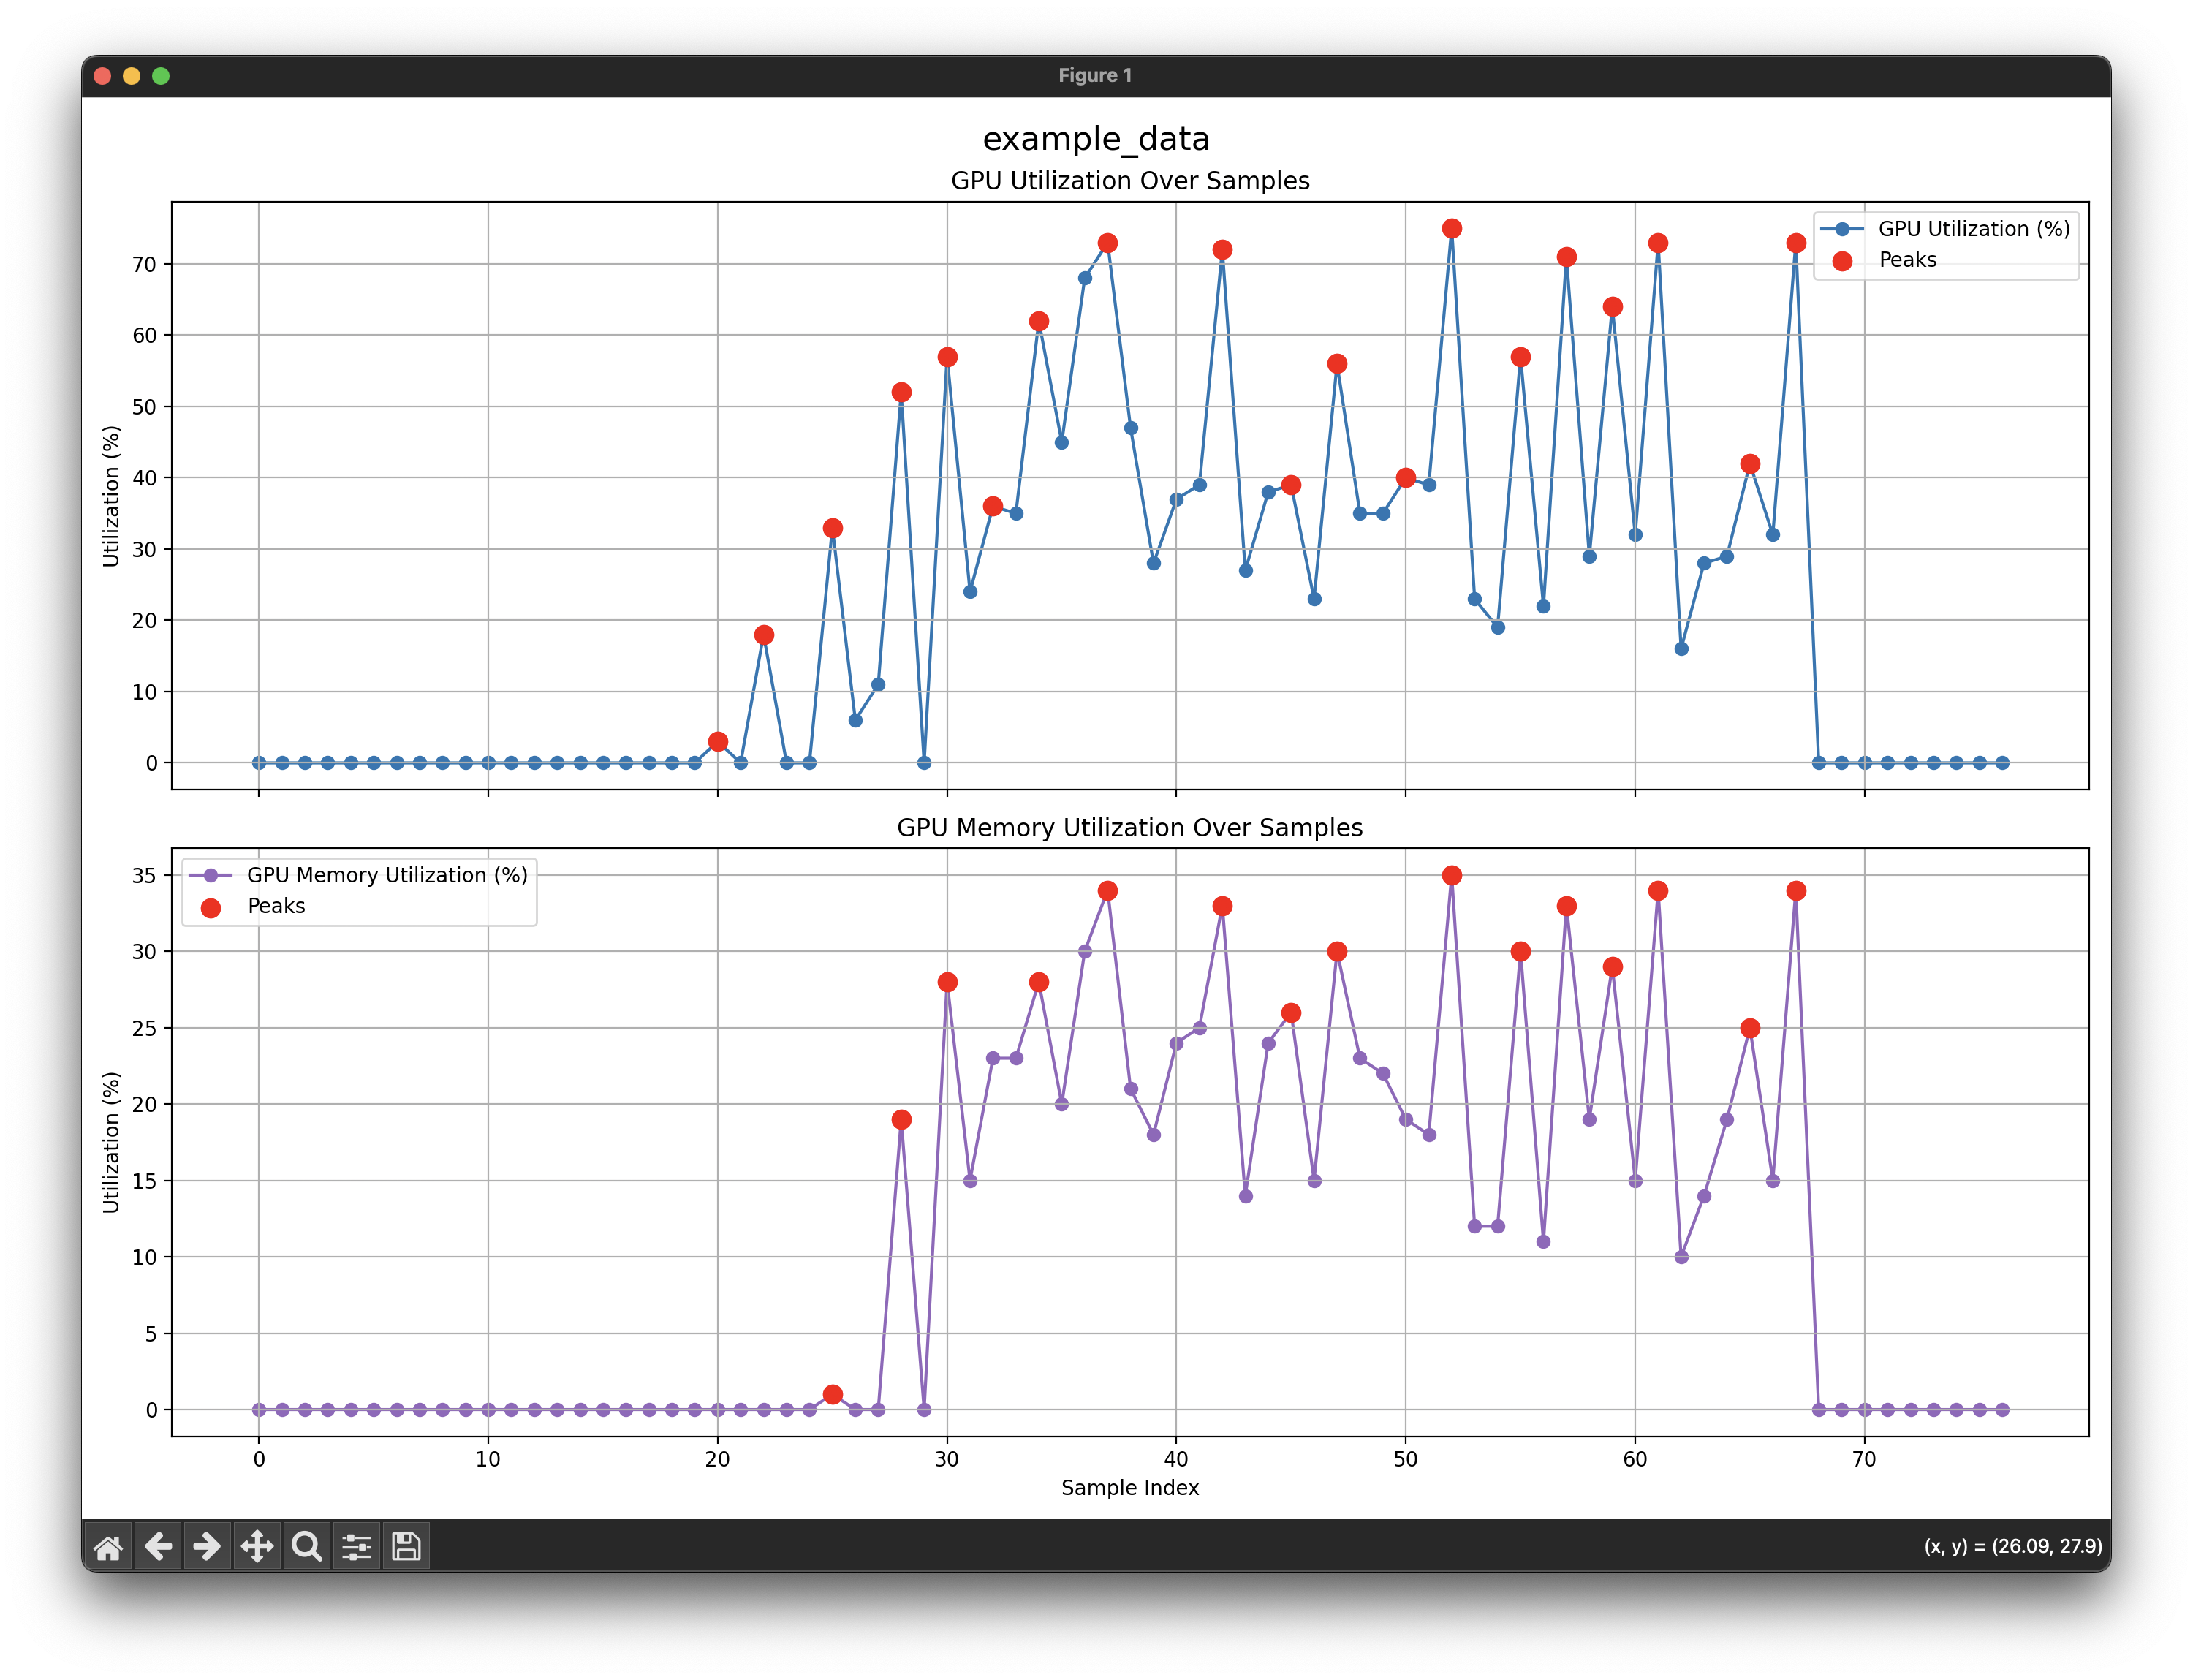
\includegraphics[width=\columnwidth]{images/profiling-example.png}
\end{figure}

% Although the integration of GPU profiling with the Alvis pipeline is mostly done, there is still some work left. While we are successfully collecting data, some (lesser important) values are currently incorrect and thus need to be addressed. Additionally, the sparse documentation as well as our limited experience with the tool means that we are not yet quite sure how to interpret all of the collected data. However, as we have mostly finished the technical integration we can now get more hands-on experience with the tool and put our focus on solving the remaining few questions before the Alvis pipeline is ready for us to start collecting the actual experiment data.

Note: we evaluated several profiling frameworks; however, the associated overhead likely distorted the performance metrics significantly. These frameworks include, but are not limited to: \href{https://github.com/gpuopenanalytics/pynvml}{pynvml}, \href{https://github.com/plasma-umass/scalene}{scalene}.

\subsection{Cosine Similarity}

We introduce a \textbf{cosine similarity} script as a ``baseline'' solution for comparison with REST-at results (i.e., a non-LLM alternative). 
% We implemented the following techniques for improving accuracy: text pre-processing, stop word removal, and TF-IDF vectorization. 
Since this algorithm produces results based on word presence and frequency, and doesn't account for the semantic meaning of the sentences, the output accuracy is directly related to how similarly the requirements and test cases are phrased in text. Table \ref{tab:cosine-baseline} presents the accuracy results across six selected datasets.

\begin{table}[h]
    \centering
    \caption{Cosine Similarity Score Baseline Accuracy}
    \renewcommand{\arraystretch}{1.2}
    \begin{tabular}{|l|c|}
    \hline
    \textbf{Dataset} & \textbf{Accuracy (\%)} \\
    \hline
    BTHS & 37.50\% \\
    ENCO & 87.50\% \\
    SnakeGame & 83.33\% \\
    Mozilla & 29.35\% \\
    HealthWatcher & 44.44\% \\
    SourceTracker & 31.82\% \\
    \hline
    \end{tabular}
    \label{tab:cosine-baseline}
\end{table}

A natural question arises: why consider this approach at all? While one might argue that leveraging LLMs for this task is excessive, our goal was to highlight significant limitations of the cosine similarity method. Specifically, it falls short when applied to larger datasets that involve diverse and complex language. 
%It thus proves the need for LLMs when working with more complex datasets since they are more suitable for extracting and interpreting the meaning of provided data. 
Thus, we prove the need for LLMs since they are more suitable for extracting and interpreting the semantic meaning in the provided data. 

\subsection{Addition of Datasets}

We include several new datasets in order to promote the validity and reliability of our results. These include: \href{https://data.mendeley.com/datasets/jw5bgshtvg/1}{Mozilla Data Source} and \href{https://zenodo.org/records/8081523}{HealthWatcher Data Source}.

We are planning to continue searching for additional datasets on the following platforms: Zenodo \& Mendeley Data, Mining Software Repositories Conference, cucumber.io, \href{https://github.com/jiwangjie/ChatBR/tree/master/questions/question1/final_sample}{Bug Reports GitHub Repository}.

\subsection{Data Sampling}

We have added a Jupyter Notebook that allows us to generate dataset subsets to be used in our experiments. Each dataset consists of three CSV files: one for requirement specifications, another for system test specifications, and the third for REST mappings. Subsets are created by randomly sampling $n$ number of requirements from the original dataset, filtering the existing dataset files based on the selected requirements, and lastly indexing and storing the filtered data in new CSV-files. 
% Currently, we have included two sampling functions that each deal with selected REST links a bit differently:

% \begin{itemize}
%     \item Option 1 ``advanced'': recursively includes all $1:n$ and $n:m$ mappings between requirements and tests that are \textit{indirectly} connected to the original sample,
%     \item Option 2 ``simpler'': only includes the original sample of requirements as well as the directly connected tests.
% \end{itemize}

% The first alternative was introduced in order to ensure that subsets do not strictly include one-to-one mappings. However, as this approach can result in subset sample sizes that may vary from what was initially specified, we will further discuss methods to achieve this goal with our supervisor and adjust the logic accordingly. One possible alternative is to introduce a more complex stratified sampling strategy, which would allow us to keep sample sizes uniform across multiple subsets and guarantee that we include one-to-many and many-to-many mappings. Regardless of our approach, the significant differences in dataset sizes coupled with the low ratios of mapping schemes other than one-to-one is presenting us with an obstacle which we will need to solve.

\subsection{Data Processing / Statistical Analysis}

To compliment the existing scripts that already evaluate the LLM-generated REST trace links, we have added code that enables us to load data from multiple sources and combine the data into dataframes. As of right now, we have the logic to generate a few different \textit{MVP}-versions of tables that showcase the overall results between different treatments for all relevant metrics. See Figure \ref{MVP-table} for an example of such a table, containing some placeholder data.

\begin{figure}[ht]
    \centering
    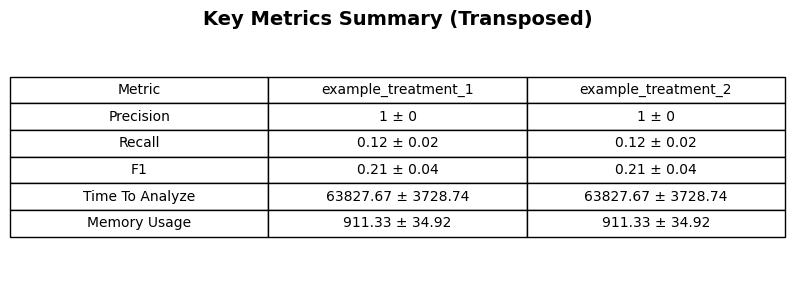
\includegraphics[width=1\linewidth]{images/MVP table example.png}
    \caption{MVP table showing mean $\pm$ standard deviation for all key metrics}
    \label{MVP-table}
\end{figure}

\textbf{Please note} that the final versions of all tables and graphs will be made more visually appealing compared to the aforementioned MVP table.

%The data analysis code will be expanded as we run our experiments and identify what statistical tests we need to conduct as well as what types of tables and plots we will need in order to effectively visualize the results. We will also spend time to make these more visually appealing compared to the MVP version just mentioned.

%Additionally, we need to modify the data processing pipeline to conform with the new output directory structure, which was introduced alongside the Alvis pipeline scripts (described in section \ref{sec:progress-alvis-pipeline}). This is likely to be fixed using a smaller Python script that will pre-process the raw output data transforming it into the format that the existing \verb|eval.py| script expects. 


\subsection{Miscellaneous Instrumentation Changes}
\begin{itemize}
    \item Updated the \verb|eval.py| script to correctly handle and generate statistics for the additional metrics related to \textbf{RQ2} (i.e., GPU memory usage and time-to-analyze).
    \item Added support for \verb|nvidia-smi| when running a job as a separate background ``monitoring'' process which can be retrieved from the REST-at core directly.
    \item Updated the \verb|send_data.py| script to accommodate for the new Alvis pipeline functionality. Added new parameters: \verb|quant|, \verb|log_dir|. Also, refactored constructing data and model paths to retrieve a corresponding environment variables in a streamlined way.
\end{itemize}

\section*{Acknowledgment}
We dedicate our gratitude to our supervisor Francisco Gomes de Oliveira Neto and our examiner Jennifer Horkoff for their valuable insights. Moreover, we are thankful for the computing platform, Alvis, offered by the Chalmers Centre for Computational Science and Engineering.

% TODO: REMOVE - TEST TABLE
%\begin{table*}
%    \centering
%        \begin{tabular}{llllllll}
%            \toprule
%            Treatment & Accuracy & Balanced Accuracy & F1 & Recall & Precision & Time To Analyze & Memory Usage \\
%            \midrule
%            test-model & $0.85 \pm 0.0$ & $0.92 \pm 0.0$ & $0.21 \pm 0.04$ & $0.12 \pm 0.02$ & $1.0 \pm 0.0$ & $63827.67 \pm 3728.74$ & $911.33 \pm 34.92$ \\
%            \bottomrule
%        \end{tabular}
%    \caption{MVP table}
%    \label{tab:my_label}
%\end{table*}

% Subsection: Results(?)
% We reassess the existing tool and make minor modifications to ensure compliance
% with the latest framework requirements and improve code readiness. This updated
% version is referred to as ``revised'' \verb|REST-at|\footnote{This version of
% the tool can be accessed via \url{https://github.com/SEM25-BSc/REST-at}.
% A complete list of changes is noted below, cf. \ref{method}.}.
% Subsection: Discussion / Results
%
% Write about Scalability? How does it perform with 10, 20, 50, 100, entries?
%
% MENTION QUANTIZATION STRICTNESS -if we pair wise the base-model with the
% quantized models, assuming the quant models have more "aggressive" quantization
% applied, we could identify the "drop-off" point, i.e., when the quantized models
% start to significantly perform worse --- useful if they perform equally well up
% until some point 

% =*= USE LATER SECTION =*=

\bibliographystyle{IEEEtran}
\bibliography{lib}

% FIXME: appendix should NOT follow double-column.
\section*{Appendix}\label{appendix}

\textit{(Left intentionally blank)}

\end{document}